%%%%%%%%%%%%%%%%%%%%%%%%%%%%%%%%%%%%%%%%%%%%%%%%%%%%%%%%%%%%%%%%%%%%%%%%%%%%%%%%%%%
%% This project aims to create the UFC template for presentation.                %%
%% author: Maurício Moreira Neto - Doctoral student in Computer Science (MDCC)   %%
%% contacts:                                                                     %%
%%    e-mail: maumneto@ufc.br                                                    %%
%%    linktree: https://linktr.ee/maumneto                                       %%
%%%%%%%%%%%%%%%%%%%%%%%%%%%%%%%%%%%%%%%%%%%%%%%%%%%%%%%%%%%%%%%%%%%%%%%%%%%%%%%%%%%
\documentclass{libs/ufc_format}
% Inserting the preamble file with the packages
%%%%%%%%%%%%%%%%%%%%%%%%%%%%%%%%%%%%%%%%%%%%%%%%%%%%%%%%%%%%%%%%%%%%%
%% This file contains the packages that can be used in the beamer. %%
%%%%%%%%%%%%%%%%%%%%%%%%%%%%%%%%%%%%%%%%%%%%%%%%%%%%%%%%%%%%%%%%%%%%%
% Package to fonts family
\usepackage[T1]{fontenc}
% Package to accentuation
\usepackage[utf8]{inputenc}
% Package to Portuguese language
\usepackage[brazil]{babel}
% Package to Figures
\usepackage{graphicx}
% Package to the colors
\usepackage{color}
% Package to the colors
\usepackage{xcolor}
% Packages to math symbols and expressions
\usepackage{amsfonts, amssymb, amsmath}
% Package to multiple lines and columns in table
\usepackage{multirow, array} 
% Package to create pseudo-code
% For more detail of this package: http://linorg.usp.br/CTAN/macros/latex/contrib/algorithm2e/doc/algorithm2e.pdf
\usepackage{algorithm2e}
% Package to insert code
\usepackage{listings} 
\usepackage{keyval}
% Package to justify text
\usepackage[document]{ragged2e}
% Package to manage the bibliography
\usepackage[backend=biber, style=numeric, sorting=none]{biblatex}
% Package to facilities quotations
\usepackage{csquotes}
% Package to use multicols
\usepackage{multicol}

% Packages added by me
\usepackage{url}
\usepackage{tikz}
%\usepackage{multimedia}
%\usepackage{media9}[playbutton=plain, windowed=1280x720]
% Inserting the references file
\bibliography{references.bib}
\renewcommand*{\bibfont}{\scriptsize}

% Title
\title[Introdução a IA]{\huge\textbf{Introdução à Inteligência Artificial}}
% Subtitle
\subtitle{Parte 4\\Tópico em Aprendizagem de Máquina}
% Author of the presentation
\author{Evandro J.R. Silva}
% Institute's Name
\institute[Estácio Teresina]{
    % email for contact
    \normalsize{\email{ejrs.profissional@gmail.com}}
    \newline
    % Department Name
    %\department{Bacharelado em Ciência da Computação}
    \newline
    % university name
    %\ufc
    \estaciothe
}
% date of the presentation
\date{30 e 31 de Janeiro}


%%%%%%%%%%%%%%%%%%%%%%%%%%%%%%%%%%%%%%%%%%%%%%%%%%%%%%%%%%%%%%%%%%%%%%%%%%%%%%%%%%
%% Start Document of the Presentation                                           %%               
%%%%%%%%%%%%%%%%%%%%%%%%%%%%%%%%%%%%%%%%%%%%%%%%%%%%%%%%%%%%%%%%%%%%%%%%%%%%%%%%%%
\begin{document}
% insert the code style
%%%%%%%%%%%%%%%%%%%%%%%%%%%%%%%%%%%%%%%%%%%%%%%%%%%%%%%%%%%%%%%%%%%%%%%%%%%%%%%%%%%
%% This file contains the style of the codes show in slides.                     %%
%% The package used is listings, but it possible to used others.                 %%
%%%%%%%%%%%%%%%%%%%%%%%%%%%%%%%%%%%%%%%%%%%%%%%%%%%%%%%%%%%%%%%%%%%%%%%%%%%%%%%%%%%

% color used in the code style
\definecolor{codegreen}{rgb}{0,0.6,0}
\definecolor{codegray}{rgb}{0.5,0.5,0.5}
\definecolor{codepurple}{rgb}{0.58,0,0.82}
\definecolor{codebackground}{rgb}{0.95,0.95,0.92}

% style of the code!
\lstdefinestyle{codestyle}{
    backgroundcolor=\color{codebackground},   
    commentstyle=\color{codegreen},
    keywordstyle=\color{magenta},
    numberstyle=\tiny\color{codegray},
    stringstyle=\color{codepurple},
    basicstyle=\ttfamily\footnotesize,
    frame=single,
    breakatwhitespace=false,         
    breaklines=true,                 
    captionpos=b,                    
    keepspaces=true,                 
    numbers=left,                    
    numbersep=5pt,                  
    showspaces=false,                
    showstringspaces=false,
    showtabs=false,                  
    tabsize=2,
    title=\lstname 
}

\lstset{style=codestyle}


%% ---------------------------------------------------------------------------
% First frame (with tile, subtitle, ...)
\begin{frame}{}
    \maketitle
\end{frame}

%% ---------------------------------------------------------------------------
% Second frame
\begin{frame}{Sumário}
    \begin{multicols}{2}
        \tableofcontents
    \end{multicols}
\end{frame}

%=============================================================================
% SECTION 1
%=============================================================================
\section{Aprendizagem de Máquina}

\begin{frame}{}
    \begin{tikzpicture}[remember picture, overlay]
        \node[anchor=north] at ([yshift=-0.45cm]current page.north)
        {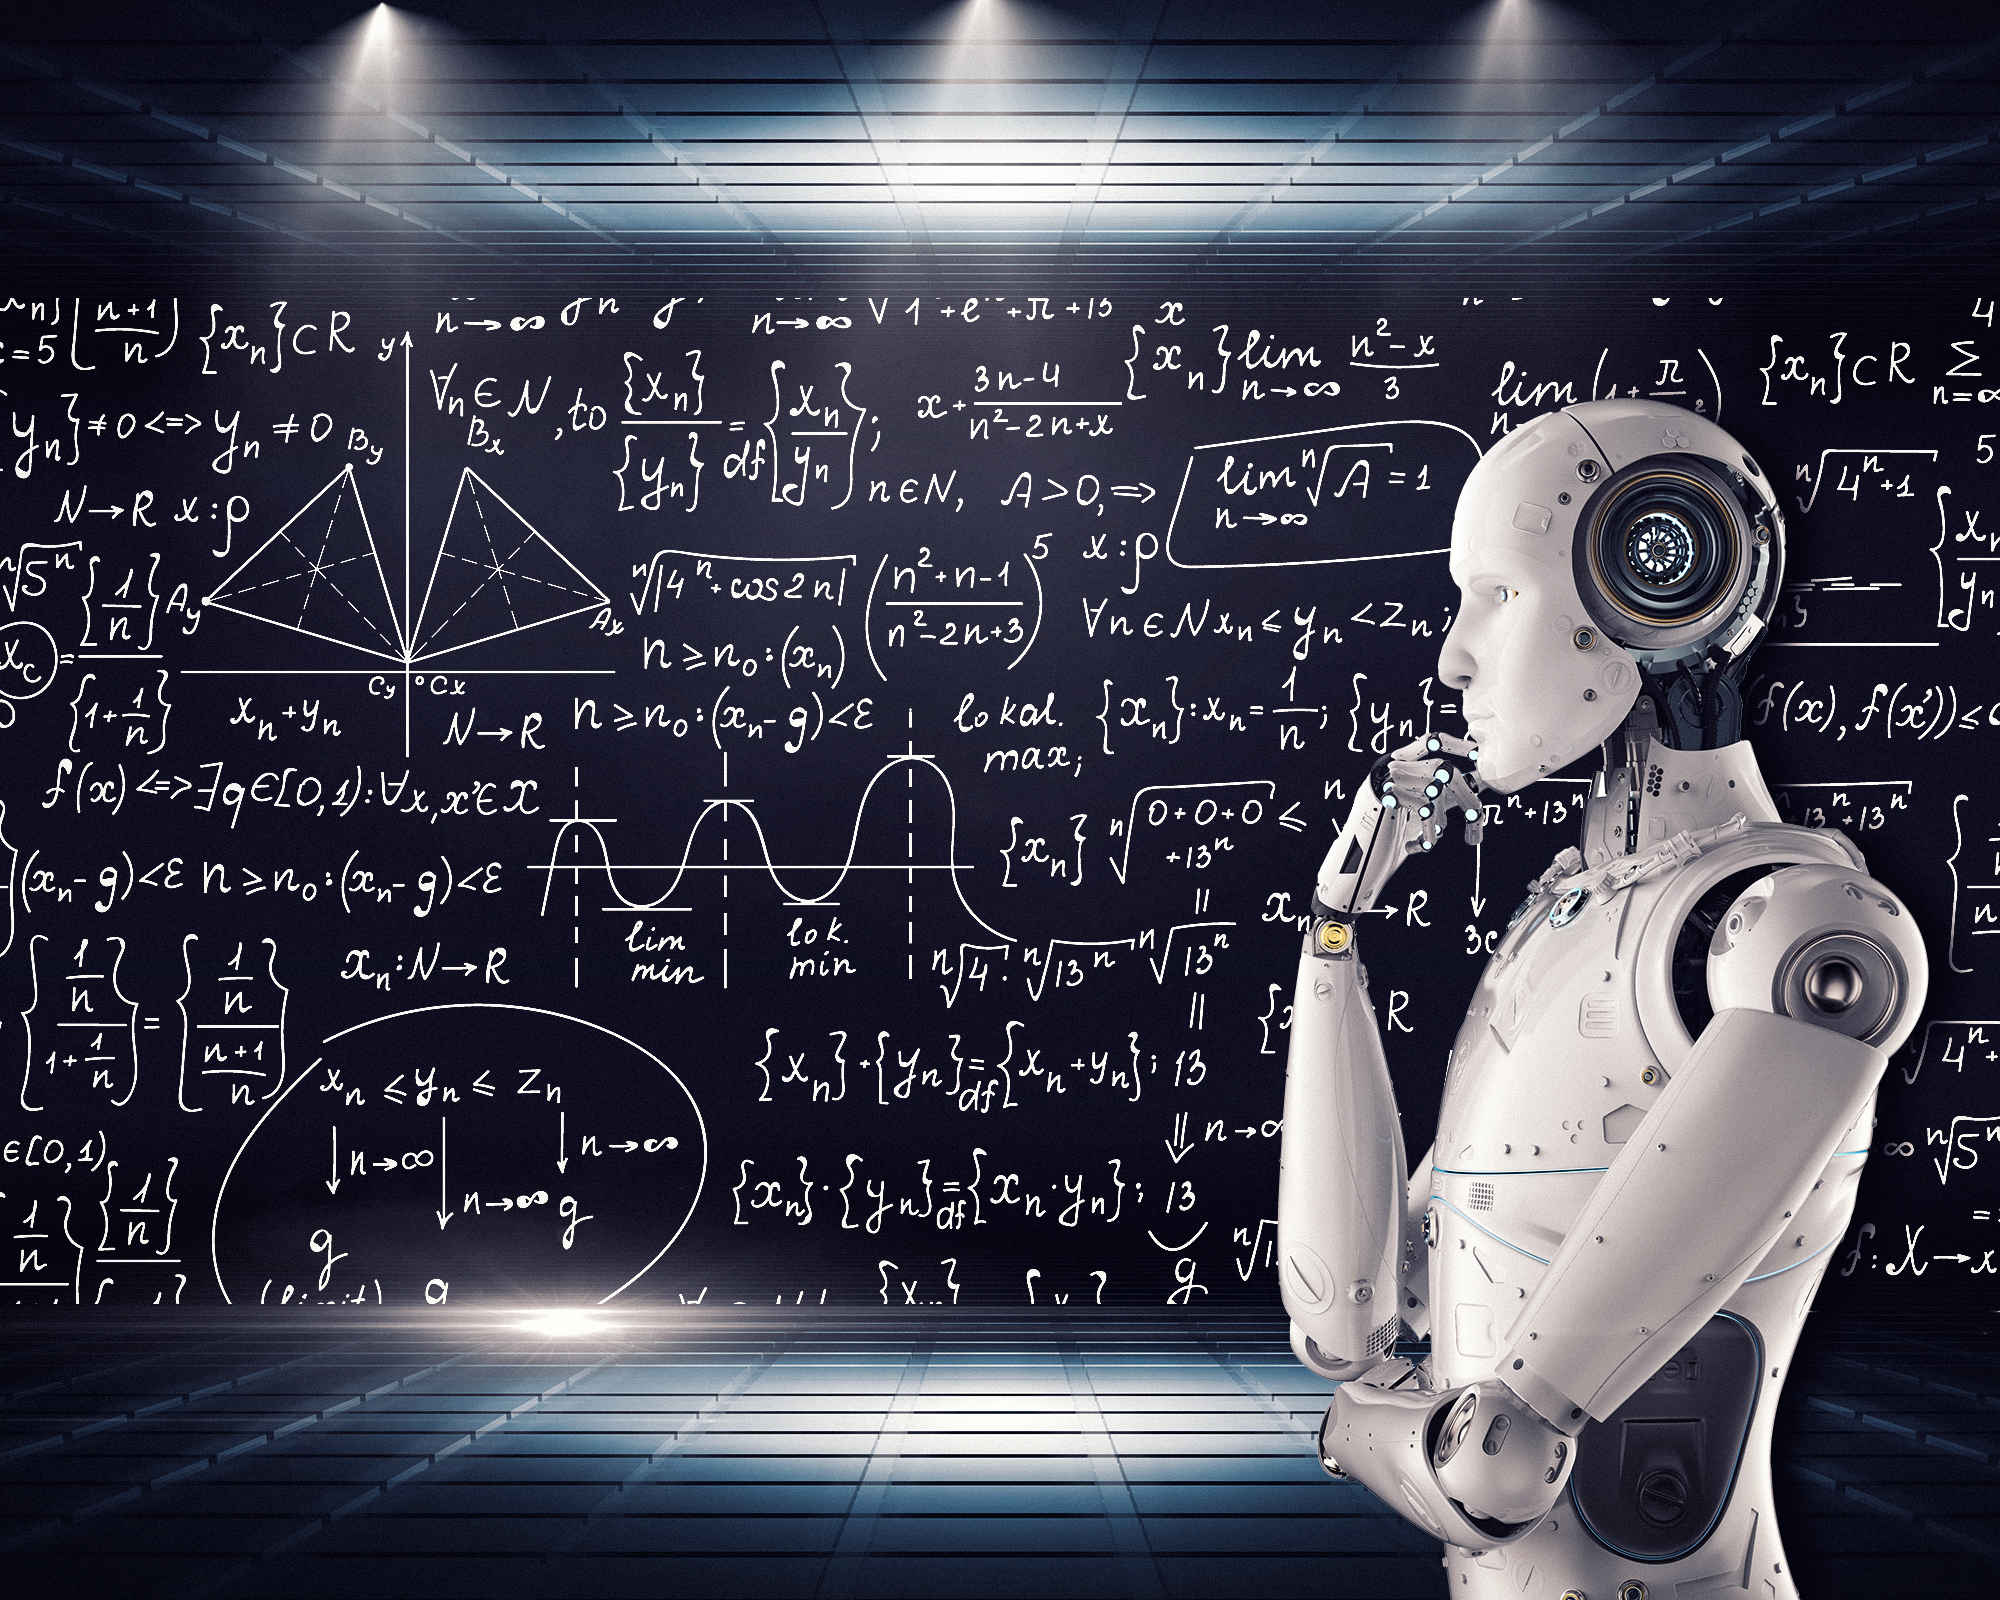
\includegraphics[width = \paperwidth]{media/robo_quadro}};
    \end{tikzpicture}
\end{frame}

\begin{frame}{Aprendizagem de Máquina (AM)}
    \begin{itemize}
        \justifying
        \item O que é aprendizado?
        \item Como aprender?
    \end{itemize}
\end{frame}

\begin{frame}{Aprendizagem de Máquina (AM)}
    \begin{itemize}
        \justifying
        \item Como você aprendeu a andar?
        \item Como você aprendeu a falar?
        \item Como você aprendeu matemática, física, química, geografia, história?
        \item Como você aprende computação?
        \item Como você aprendeu a diferenciar um rosto de outro?
        \item Como você aprendeu a diferenciar uma música de outra?
    \end{itemize}
    
    \tikz[remember picture,overlay] \node[opacity=0.2,inner sep=0pt] at (current page.center){
\includegraphics[width=\paperwidth,height=\paperheight]{memes/dieMeme}};
\end{frame}

\begin{frame}{Aprendizagem de Máquina (AM)}
    \begin{block}{Definição de AM}
        \justifying
        Um programa de computador aprende de uma experiência $E$ com respeito a algum conjunto de tarefas $T$ e uma medida de performance $P$, se sua performance nas tarefas em $T$, medido por $P$ melhora com a experiência $E$ \cite{m97}.
    \end{block}
\end{frame}

\begin{frame}{Aprendizagem de Máquina (AM)}
    \begin{itemize}
        \item<1> Exemplo 1
            \begin{itemize}
                \justifying
                \item<1> Tarefefa $T$: jogar xadrez.
                \item<1> Medida de performance (desempenho) $P$: porcentagem de jogos ganhos contra oponentes.
                \item<1> Experiência de treino $E$: praticar em partidas consigo mesmo.
            \end{itemize}
        \item<2> Exemplo 2
            \begin{itemize}
                \item<2> Tarefa $T$: dirigir um carro usando os sensores.
                \item<2> Medida de desempenho $P$: distância média percorrida antes de algum erro ou acidente.
                \item<2> Experiência de treino $E$: sequência de imagens e manipulações do veículo feitas por um humano.
            \end{itemize}
    \end{itemize}
\end{frame}

\begin{frame}{Aprendizagem de Máquina (AM)}
\centering
\large
Vídeo do Two Minute Papers \cite{tmp19}
\end{frame}

%-----------------------------------------------------------------------------
% SUBSECTION 1.1
%-----------------------------------------------------------------------------
\subsection{Tipos de Aprendizado}

\begin{frame}{Tipos de Aprendizado}
    \begin{itemize}
        \justifying
        \item Existem três tipos básicos de aprendizado: \alert<2>{\textbf{Supervisionado}}, \textbf{Não Supervisionado} e \textbf{Por Reforço}.
    \end{itemize}
\end{frame}

\begin{frame}{Tipos de Aprendizado}
    \begin{itemize}
        \item Aprendizado Supervisionado
            \begin{itemize}
                \justifying
                \item Possivelmente o mais comum.
                \item É chamado de supervisionado porque as \textit{saídas} são conhecidas e fornecidas ao algoritmo de aprendizado.
                \item É como se houvesse um professor para corrigir os erros $\rightarrow$ o professor sabe a resposta correta.
            \end{itemize}
    \end{itemize}
\end{frame}

\begin{frame}{Tipos de Aprendizado}
    \begin{itemize}
        \item Aprendizado Supervisionado
            \begin{itemize}
                \justifying
                \item De uma maneira mais formal, o aprendizado supervisionado cria um modelo matemático que retorna uma resposta para um determinado conjunto de entradas.
                \item Como o modelo matemático vai sendo construído:
                    \begin{enumerate}
                        \justifying
                        \item<2> Um conjunto de dados é dividido em três subconjuntos: \textbf{treinamento}, \textbf{validação} e \textbf{teste}.
                        \item<3> O algoritmo recebe as entradas de cada observação do conjunto de treinamento e devolve uma saída/resposta.
                        \item<4> Conferimos cada resposta do algoritmo com a resposta correta. Se a resposta do algoritmo estiver errada, o algoritmo é informado do erro.
                        \item<5> Ao terminar de treinar com todos os dados de treinamento, o algoritmo verifica o quão bom está gerando respostas para os dados de validação. Se o algoritmo ainda está ruim, então fazemos um novo treinamento. Senão, vamos direto aos testes.
                    \end{enumerate}
            \end{itemize}
    \end{itemize}
\end{frame}

\begin{frame}{Tipos de Aprendizado}
    \begin{itemize}
        \item Aprendizado Supervisionado
            \begin{itemize}
                \justifying
                \item É utilizado para duas tarefas principais: \alert<2>{classificação} e \alert<3>{regressão}.
                \item<2> Uma máquina passa a ser capaz de classificar alguma coisa a partir da observação dos atributos.
                \item<3> Estimação da relação entre uma variável dependente e uma ou mais variáveis independentes.
            \end{itemize}
    \end{itemize}
\end{frame}

\begin{frame}{Tipos de Aprendizado}
    \centering
    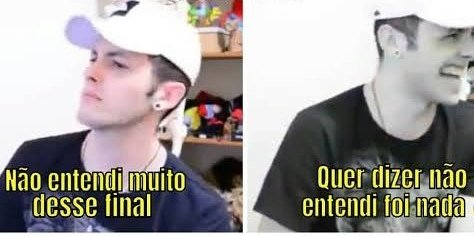
\includegraphics[width=\textwidth]{memes/entendi_nada}
\end{frame}

%- - - - - - - - - - - - - - - - - - - - - - - - - - - - - - - - - - - - - - -
% SUBSUBSECTION 1.1.1
%- - - - - - - - - - - - - - - - - - - - - - - - - - - - - - - - - - - - - - -
%\subsubsection{Classificação}

\begin{frame}{Aprendizado Supervisionado  --- Classificação}
    \begin{figure}
        \centering
        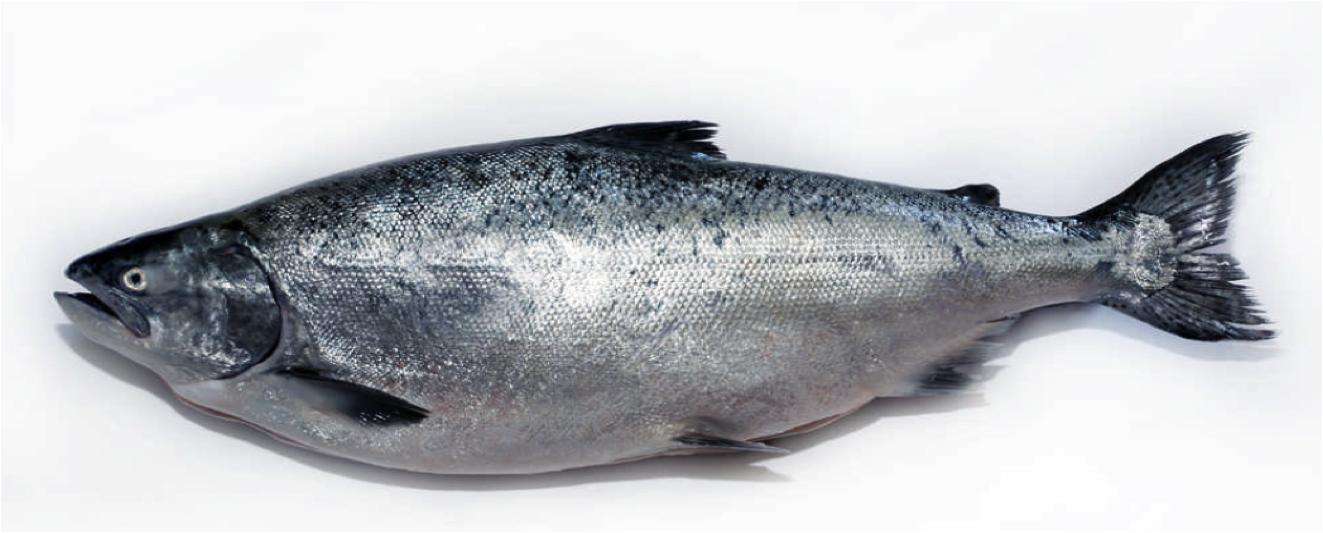
\includegraphics[width=6.5cm]{media/salmon}
        \caption{Salmão}
        \label{fSalmao}
    \end{figure}
    \vspace{-0.5cm}
    \begin{figure}
        \centering
        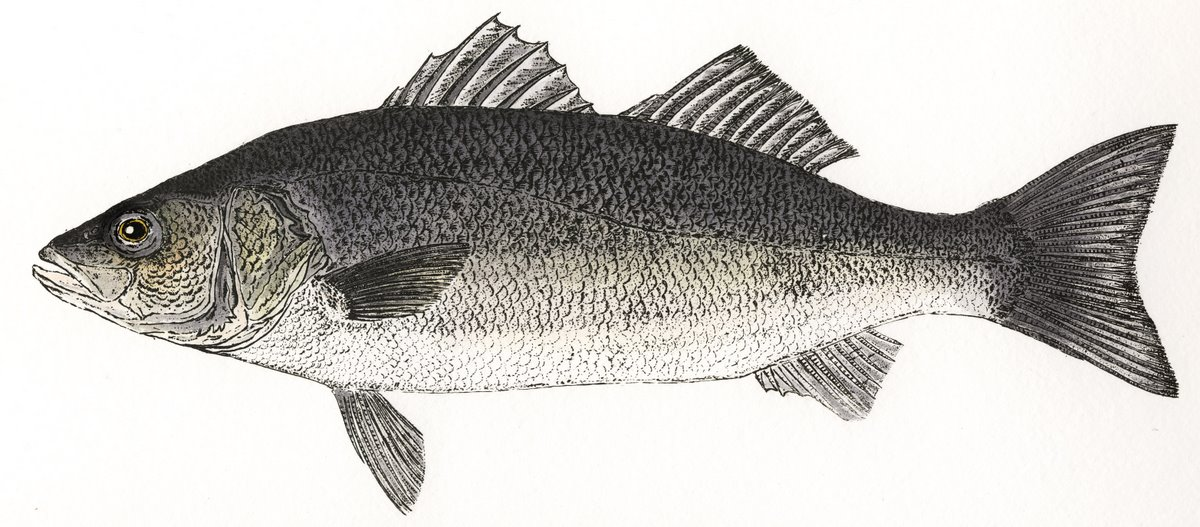
\includegraphics[width=6.5cm]{media/seabass}
        \caption{Robalo}
        \label{fRobalo}
    \end{figure}
\end{frame}

\begin{frame}{Aprendizado Supervisionado  --- Classificação}
    \begin{itemize}
        \justifying
        \item Suponha os seguintes atributos: brilho das escamas e comprimento das barbatanas.
        \item Para cada foto/observação, um valor é atribuído aos atributos.
        \item A partir dos valores dos atributos uma máquina pode aprender como classificar um peixe ainda não visto.
    \end{itemize}
\end{frame}

%- - - - - - - - - - - - - - - - - - - - - - - - - - - - - - - - - - - - - - -
% SUBSUBSECTION 3.1.2
%- - - - - - - - - - - - - - - - - - - - - - - - - - - - - - - - - - - - - - -
%\subsubsection{Regressão}

\begin{frame}{Aprendizado Supervisionado  --- Regressão}
    \begin{itemize}
        \justifying
        \item A partir de um conjunto de dados, com a regressão você consegue criar uma função que se aproxime ao observado.
        \item É comumente utilizado para predição, ou análise temporal.
    \end{itemize}
    \centering
    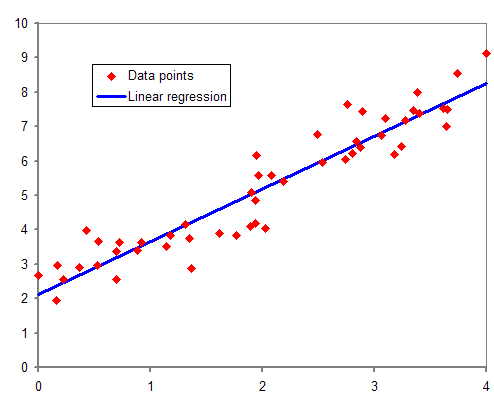
\includegraphics[scale = 0.45]{media/normdist_regression}
\end{frame}

\begin{frame}{Tipos de Aprendizado}
    \begin{itemize}
        \justifying
        \item Voltando aos tipos de aprendizado: \textbf{Supervisionado}, \alert{\textbf{Não Supervisionado}} e \textbf{Por Reforço}.
    \end{itemize}
\end{frame}

\begin{frame}{Tipos de Aprendizado}
    \begin{itemize}
        \item Aprendizado Não Supervisionado
            \begin{itemize}
                \justifying
                \item Neste tipo de aprendizado não existe a figura do \textit{professor}.
                \item<2-> O algoritmo não tem como saber se está certo ou errado.
                \item<3-> O aprendizado acontece puramente por \textit{experiência}.
                \item<4-> O algoritmo vai analisar os dados e tentar fazer alguma \alert<5>{inferência} a partir dos atributos.
                \item<5> Uma das aplicações mais comum é organizar os dados de acordo com sua similaridade (\textit{clustering}, ou agrupamento).
            \end{itemize}
    \end{itemize}
\end{frame}

\begin{frame}{Tipos de Aprendizado}
    \begin{itemize}
        \item Aprendizado Não Supervisionado
    \end{itemize}
    \centering
    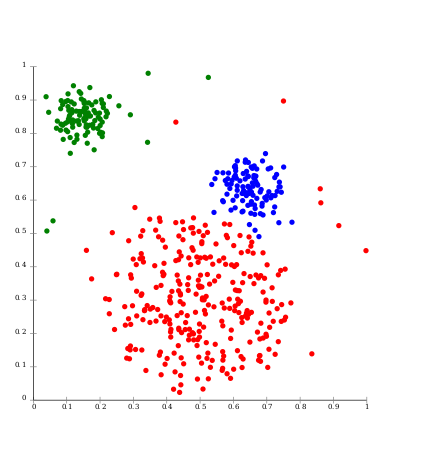
\includegraphics[scale=0.45]{media/optics_gaussian_data}
\end{frame}

\begin{frame}{Tipos de Aprendizado}
    \begin{itemize}
        \item Aprendizado Não Supervisionado
    \end{itemize}
    \centering
    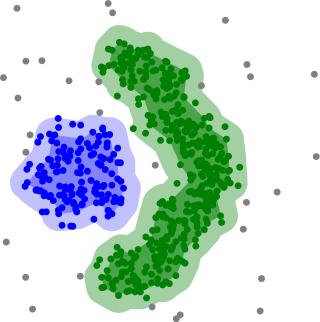
\includegraphics[scale=0.45]{media/dbscan_density_data}
\end{frame}

\begin{frame}{Tipos de Aprendizado}
    \begin{itemize}
        \item Aprendizado Por Reforço
            \begin{itemize}
                \justifying
                \item O tipo de aprendizado menos comum.
                \item<2-> Consiste em dar uma \textit{recompensa} ao algoritmo quando ele acerta, ou uma \textit{penalidade} quando erra.
                \item<3-> A diferença principal para o Aprendizado Supervisionado é que agora o algoritmo não sabe o quanto está certo ou errado.
            \end{itemize}
    \end{itemize}
\end{frame}
%=============================================================================
% SECTION ?
%=============================================================================
\section{FIM}

\begin{frame}{}
    \centering
    \Large
    Terminamos a Terceira Parte!\\
    Obrigado pela atenção!
\end{frame}

%=============================================================================
% SECTION REFERENCES
%=============================================================================
\begin{frame}[allowframebreaks]{Referências}
    \scriptsize
    \printbibliography
\end{frame}

\end{document}













%% ---------------------------------------------------------------------------
% This presentation is separated by sections and subsections
%\section{Seção I}
%\begin{frame}{Explicações}
%    % itemize
%    Este é um template que pode ser utilizado para:
%    \begin{itemize}
%        \item Apresentação de Trabalhos Acadêmicos
%        \item Apresentação de Disciplinas
%        \item Apresentações de Teses e Dissertações
%    \end{itemize}
%
%    \vspace{0.4cm} % vertical space
%    
%    % enumeration
%    Para utilizar este template corretamente é importante que:
%    \begin{enumerate}
%        \item Tenha conhecimento mínimo sobre LaTeX
%        \item Ler os comentários no template (explicações)
%        \item Ler o README.md (documentação)
%    \end{enumerate}
%
%    \vspace{0.2cm}

%    \example{Este é um texto de exemplo!} \emph{Texto de Ênfase!}
%\end{frame}

%% ---------------------------------------------------------------------------
%\subsection{Subseção I}
%\begin{frame}{Criando Blocos}
%    % Blocks styles
%    \begin{block}{Bloco Padrão}
%        Texto do corpo do bloco.
%    \end{block}

%    \begin{alertblock}{Bloco de Alerta}
%        Texto do corpo do bloco.
%    \end{alertblock}
%
%    \begin{exampleblock}{Bloco de Exemplo}
%        Texto do corpo do bloco.
%    \end{exampleblock}   
%\end{frame}

%% ---------------------------------------------------------------------------
%\subsection{Subseção II}
%\begin{frame}{Criando Caixas}
%    \successbox{testando o success box}
%
%    \pause
%
%    \alertbox{testando o alert box}
%
%    \pause
%
%    \simplebox{testando o simple box}
%\end{frame}

%% ---------------------------------------------------------------------------
%\subsection{Subseção III}
%\begin{frame}{Criando Algoritmos (Pseudocódigo)}
%    \begin{algorithm}[H]
%        \SetAlgoLined
%        \LinesNumbered
%        \SetKwInOut{Input}{input}
%        \SetKwInOut{Output}{output}
%        \Input{x: float, y: float}
%        \Output{r: float}
%        \While{True}{
%          r = x + y\;
%          \eIf{r >= 30}{
%           ``O valor de $r$ é maior ou iqual a 10.''\;
%           break\;
%           }{
%           ``O valor de $r$ = '', r\;
%          }
%         } 
%         \caption{Algorithm Example}
%    \end{algorithm}
%\end{frame}

%% ---------------------------------------------------------------------------

%\begin{frame}{Inserindo Algoritmos}
%    \lstset{language=Python}
%    \lstinputlisting[language=Python]{code/main.py}
%\end{frame}

%% ---------------------------------------------------------------------------
%\begin{frame}{Inserindo Algoritmos}
%    \lstinputlisting[language=C]{code/source.c}
%\end{frame}

%% ---------------------------------------------------------------------------
%\begin{frame}{Inserindo Algoritmos}
%    \lstinputlisting[language=Java]{code/helloworld.java}
%\end{frame}

%% ---------------------------------------------------------------------------
%\begin{frame}{Inserindo Algoritmos}
%    \lstinputlisting[language=HTML]{code/index.html}
%\end{frame}

%% ---------------------------------------------------------------------------
% This frame show an example to insert multicolumns
%\section{Multicolunas}
%\begin{frame}{Seção II - Multicolunas}
%    \begin{columns}{}
%        \begin{column}{0.5\textwidth}
%            \justify
%            É possível colocar mais de uma coluna utilizando os comandos de $\backslash$begin\{column\}\{\} e $\backslash$end\{column\}
%        \end{column}
%        \begin{column}{0.5\textwidth}
%            \justify
%            Porém, o espaçamento deve ser proporcional entre as colunas para que estas colunas não entrem em coflito. O espaçamento é dado pelo segundo argumento do $\backslash$begin.
%        \end{column}
%    \end{columns}    
%\end{frame}

%% ---------------------------------------------------------------------------
% This frame show an example to insert figures
%\section{Imagens}
%\begin{frame}{Seção III - Figures}
%    \begin{figure}
%        \centering
%        \caption{Emblema da UFC.}
%        
\includegraphics[scale=0.3]{libs/emblemufc.pdf}
%        \source{Obtido pelo site oficial da UFC \cite{siteufc} \cite{einstein}}
%        \label{fig:ufc_emblem}
%    \end{figure}
%\end{frame}

%% ---------------------------------------------------------------------------
% Reference frames
%\begin{frame}[allowframebreaks]
%    \frametitle{Referências}
%    \printbibliography
%\end{frame}

%% ---------------------------------------------------------------------------
% Final frame
%\begin{frame}{}
%    \centering
%    \huge{\textbf{\example{Obrigado(a) pela Atenção!}}}
%    
%    \vspace{1cm}
%    
%    \Large{\textbf{Contato:}}
%    \newline
%    \vspace*{0.5cm}
%    \large{\email{usuario@dominio}}
%\end{frame}